\documentclass[11pt, a4paper, oneside]{report}
\usepackage[utf8]{inputenc}
% \usepackage{CormorantGaramond}
\usepackage{hyperref}
\usepackage{booktabs}
\usepackage{graphicx}
\usepackage{anysize}
\graphicspath{ {./docs/} }

\hypersetup{
	colorlinks=true,
	linkcolor=black,
	filecolor=blue,
	urlcolor=black,
	pdftitle={Report on S6 project},
}

\title{\textbf{Report on the ConnAIct 4 project}}
\author{\normalsize François Barnouin, Cindy Do, Henri Gasc\\\normalsize Hamza Jad Al Aoun, Guillaume Ung\\\\\\\\\\\\\\\\\\Under the supervision of \textbf{\textit{Nicholas Evans}}}
\date{}

\begin{document}
	\marginsize{2.5cm}{2.5cm}{3cm}{3cm}
	\maketitle
	\tableofcontents

	\chapter{Introduction}
	The Connect 4 game is a classical and well-known game. It is often used as a mean to evaluate how comfortable someone is in it's programming capabilities. \\
	Today, we are the one evaluated on it, but with a few twists. We have to create an AI to play the game, communicate with another player wirelessly, and accept some signs that someone does to a camera as an input. \\
	This represents a four-way challenge.
	\begin{itemize}
		\item Firstly, we have to code the logic behind the Connect 4 in a way that makes it easy for the other parts to work with.
		\item Secondly, our AI needs to be fast, and robust.
		\item Thirdly, we have to choose some gestures, make it fast and easy to use.
		\item Last but not least, we need to define the protocols and technologies used to communicate.
	\end{itemize}

	\chapter{User manual}

	\section{Specifications}
	To use the whole project (meaning, with the camera, the AI in C++, the communication module), you need to have installed:
	\begin{itemize}
		\item A version of Python (preferably \(>=\) 3.11),
		\item A C++ compiler (\textit{clang++} produces better binary but \textit{g++} works too),
		\item A working bash interpreter,
		\item A Raspberry Pi under Raspbian64 with a camera module, a Bluetooth chip, and at least 2 GB of RAM.\@
	\end{itemize}
	All those requirements are easy to fulfil, and you should not have anything to install on your own. \\

	\section{Setting up}
	When the previous requirements are fulfilled, you only need to use the \textit{launch.sh} script, and every other software and libraries required should be installed. \\
	If the script does not find something, then it prints it and launches the program with some options disabled. \\
	If you want to use Bluetooth in server mode, then you need to run the script as root (under Linux, you just need to use \textit{sudo ./launch.sh}). It is because advertising the Bluetooth service need root permission.

	\section{Indications}
	Once the program opens, you should be able to understand easily what to do, and how to do it. However, if it is needed, here is the explanation about the different screens of the game. \\

	This first screen displays to you the menu. You may go to the options or play menu. \\
	\hspace*{1cm} In the options screen, you can choose the language you want the program to use, if you want to use the camera, if you want to have sound when playing. To change those, just click on the relevant icon. \\
	\hspace*{1cm} The play menu lets you choose if you want to play against a human, against an AI, or if you want to watch two AI battle each other for domination. When choosing a game including an AI, you will be able to select its difficulty. \\

	When playing, you can use your mouse or your hand (if you activated the camera) to select the column in which you want to put your token in. The selected column will be highlighted.

	\chapter{Technical manual}
	% A technical manual that explains:
	% \begin{itemize}
	% 	\item The design and development choices, motivates them, and optionally compares them with other possible choices.
	% 	\item The software architecture and the role of each file in the source code archive.
	% 	\item How the produced source code has been validated and verified, and with what results.
	% 	\item What difficulties have been encountered and how they have been solved.
	% \end{itemize}

	\section{Interface}
	For the interface, we chose to use Python for its ease of use. We used classes because this representation is very flexible and close to what we want. \\
	The most challenging part in writing the interface was managing to integrate the communication, AI, and gestures recognition in the code in a way that makes it easy to modify things. Using classes was a way to solve those problems before they became hindrances. \\

	Each “screen” of the game (All the menus + the game screen (with the board)) is its own class, inherited from a base class common to all screens. The basic principle to display things is the same, only the content is different. This way, a graphical continuity is preserved between all screens. \\

	Classes are made for each player, the board of the game, the gestures, the AI, and the communication, as well as for the game itself. \\
	This way, all the code is well compartmented and we can easily change how something is done in the backend as long as we don't change the API (meaning, the arguments and return statements of the functions) calls. \\

	\section{AI}\label{AI_section}

	We went through several stages while implementing the artificial intelligence. We improved the code step-by-step in order to have the best behaviour possible. \\

	\subsection{First stage, Basic functionalities}

	The first stage was very simple, we had to implement some basic functions. \\
	We decided to represent the state of a game using 64 bits numbers. This representation is called a bitboard. The presence of a token in a position is translated into a 1 in its place on the bitboard. \\
	We are using an 8 by 8 board (so that it fits into an \textit{uint64\_t} object), with the top row and right-most column always empty. Figure~\ref{fig:example_game_state} shows an example of a game state with the bitboard corresponding to the first ('x') and second ('o') player.

	\begin{figure}[ht]
		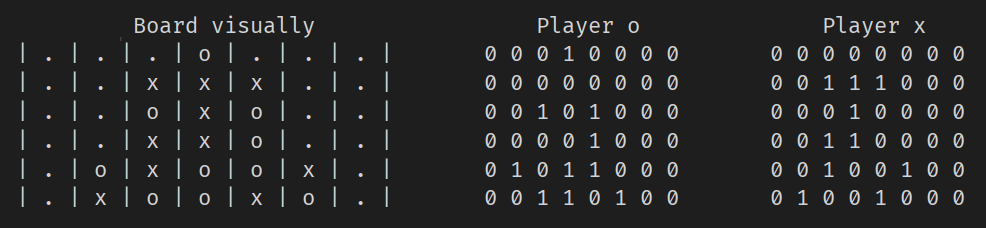
\includegraphics[scale=0.4]{example.png}
		\centering
		\caption{Example of a game state (without empty top row)}\label{fig:example_game_state}
	\end{figure}

	We started by implementing the functions that would allow us to drop a piece in a column and to scan the board in order to see if a player had won the game. At this point, by simply displaying the board, it was possible to play Connect 4 with two human players. That’s a start, but we are not quite where we want yet. \\

	\subsection{Second stage, Basic AI without foreseeing capabilities}

	We first needed to give the computer some indications, so it could understand in which column it had to play. This is the start of our first heuristic function (or evaluation function), the scoring function that determines the score of a given game state. \\
	It was using the number of tokens that were aligned in each direction (horizontally, vertically and diagonally). We implemented a scanning function which created a four positions window on the board and counted the number of tokens for both players and the number of empty spaces. A score was then deduced and given to the predicted move according to the number of two and three in a row in that window. The logic behind this being, the more points a column had, the more likely we could win using the column. \\
	Of course, the heuristic is designed in a way that if a player can win or defend from the opponent’s three in a row, it will automatically do it. \\

	This first artificial intelligence was simple, could win against player choosing a column randomly or even against very distracted players (we did ashamedly lose a couple of times). However, there was no strategy at all, we could not settle for that. We had to go further. \\

	\subsection{Third stage, Minimax algorithm}

	First, we decided to implement a decisional tree. The root of the tree is our starting game state, each branch is a possible move, and each subsecant node is the game state should we follow this path. This tree has all game states until a depth chosen before starting the exploration. There are at most 7 branches for each state, and the player playing switches at every depth. \\

	Now that we have created a structure in which the states of the boards will be represented, we have to choose the method to explore this jungle of possibilities and find the best possible path each time. For that, we used the minimax algorithm. It is a recursive algorithm which is implemented in decision-making game and game theory fields. It tries to analyse the possible paths and returns the optimal move for a player assuming that the opponent is also playing optimally. \\

	To accomplish that, there is a maximizing player (with which we try to have as many points as possible) and a minimizing player (with which we try to have as fewer points as possible). Both are using the same heuristic function. The algorithm performs a depth-first search (DFS), it will explore the complete game tree as deep as possible, all the way down to the leafs. \\
	The minimax was not hard to implement, and after this stage we had a decent AI.\@ However, the computational time was way too long, so we had to implement other features and optimizations in our code. \\

	\subsection{Fourth stage, Features and Optimizations}
	Now that we have a working algorithm, we can focus on improving it. \\

	At first, we implemented alpha-beta pruning. It introduces a score window [alpha, beta] within which the actual score of the game state is searched. Thus, we do not have to explore all paths and compute scores associated with boards we know to be worse than what we have already explored. It allows us to prune the search tree on some conditions. \\
	There are 3 possible cases:

	— The score of the position is within the window, the function returns the exact score.
	
	— The score of the position is lower than alpha, the function is allowed to return any upper bound of the actual score that is lower than or equal to alpha.

	— The score of the position is greater than beta, the function is allowed to return any lower bound of the actual score that is greater than or equal to beta. \\
	Then, several other optimizations were made:
	
	— We translated the minimax algorithm in C++ to reduce the overhead and thus the computing time,

	— We implemented column ordering: explore the columns starting from the middle and expanding one by one to the sides (usually, the middle column gives better odds at winning, thus furthering the improvements made by alpha-beta pruning),

	— We used negamax, a minimax variant make use of the zero-sum property of the game. This reduced the number of comparison needed at each step. \\

	Several other small computing time-related optimizations were made. On Figure~\ref{fig:ai_benchmarks}, you can see a graph summarizing the benchmarks of those optimizations. Step 0 is the minimax alone, step 1 is the minimax algorithm with alpha-beta pruning, step 2 is negamax with alpha-beta pruning, step 3 is column ordering in negamax, and finally step 4 is with all other optimizations. % 922252800000 nodes explored for minimax alone before being stopped at more than 2h of running
	\begin{figure}[ht]
		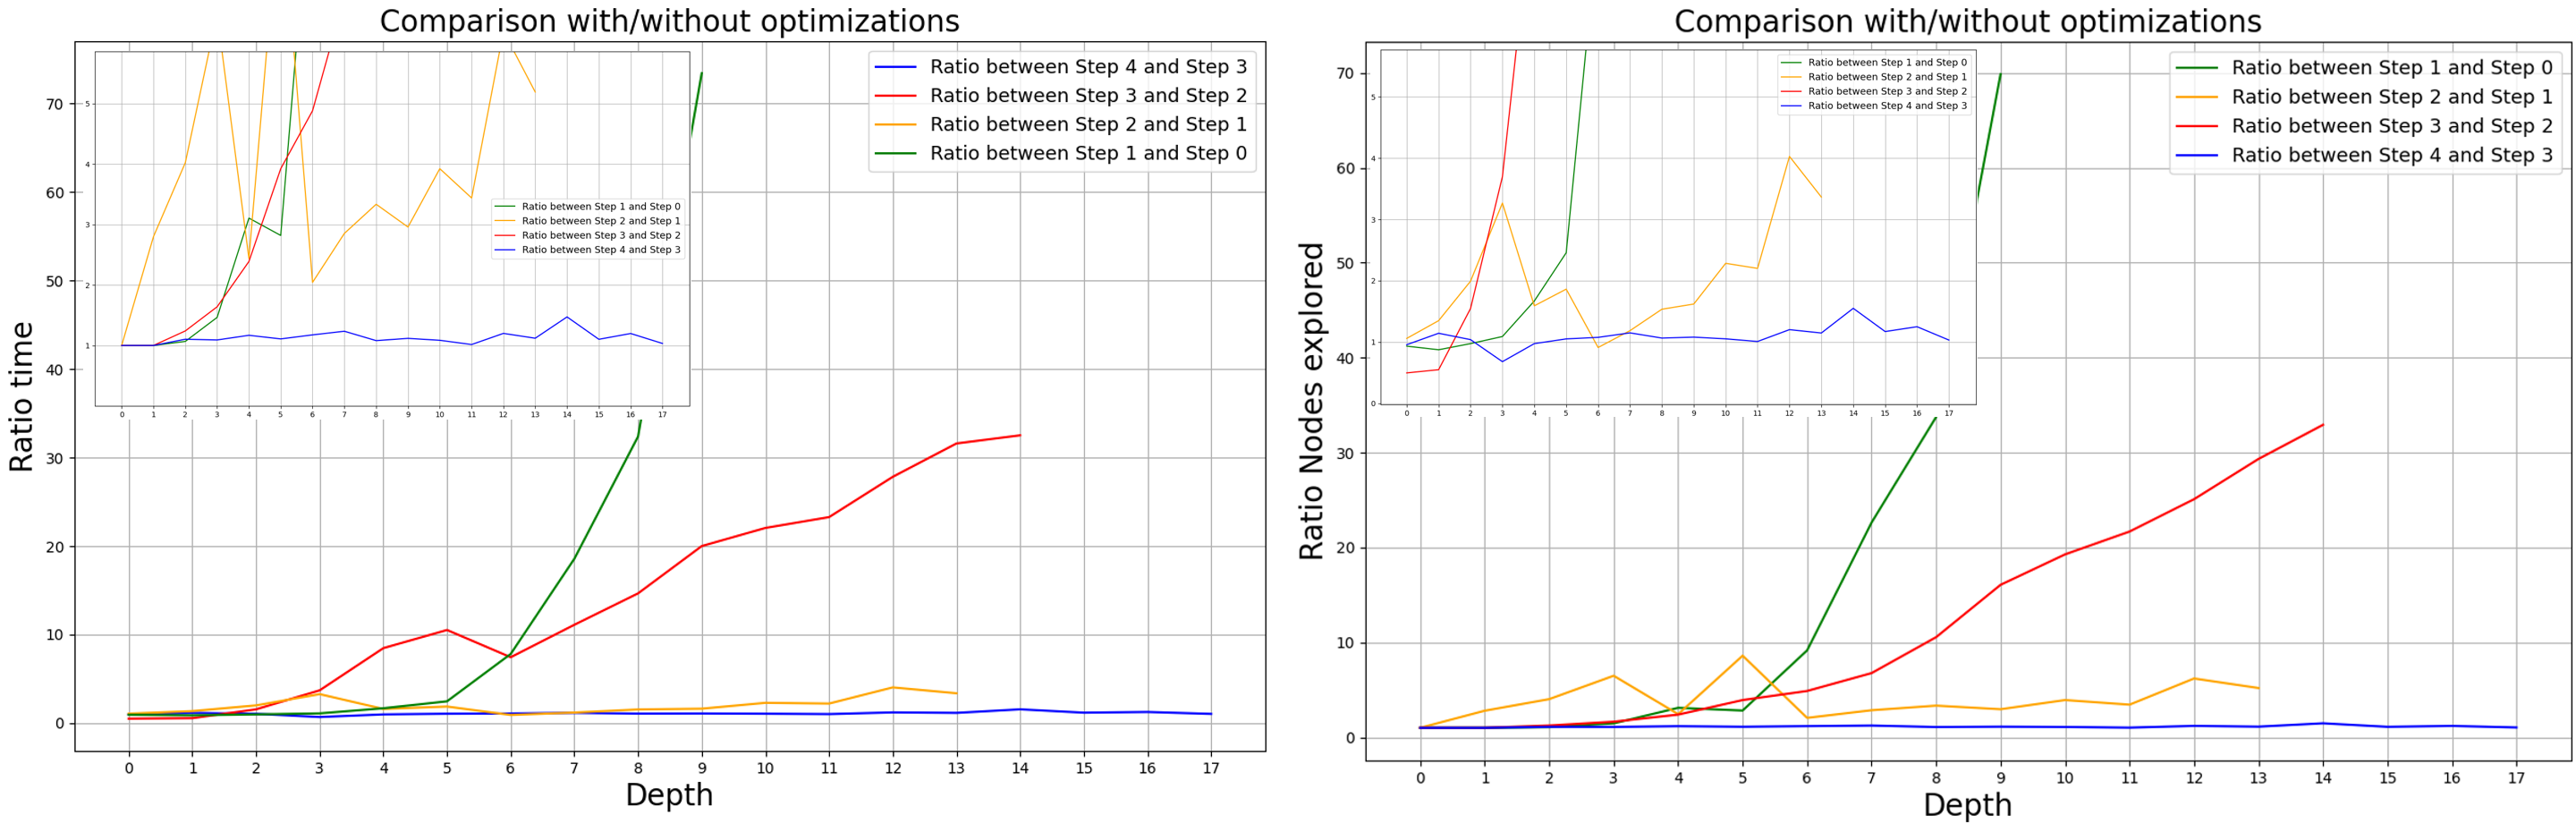
\includegraphics[scale=0.7]{Comparison_ai_stages.png}
		\centering
		\caption{Comparison between different stages.}\label{fig:ai_benchmarks}
	\end{figure}

	Finally, our artificial intelligence was made, and the deeper the level, the harder it was for us to beat it. Even when losing, it gave a truly satisfying result. But how could we judge the efficiency of our artificial intelligence ? We decided to do so by creating a small set of criteria:

	— At any depth, an AI must beat a player that is always choosing a column randomly.

	— At any depth, an AI must beat another AI with depth level strictly lower than itself.

	— Finally, for a given depth level, the AI who starts first must beat an AI with the same depth. \\

	As you can see in Figure~\ref{fig:summary_criteria}, they are not always respected (except for the 1st criterion), but most of the time it is the case.
	\begin{figure}[ht]
		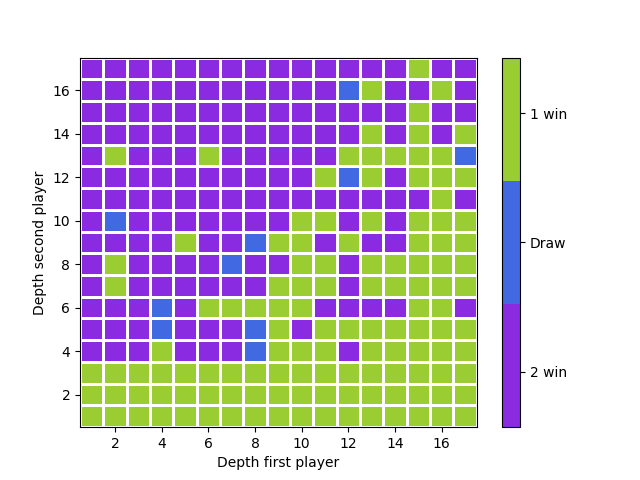
\includegraphics[scale=0.7]{result_criteria.png}
		\centering
		\caption{Summary of the evaluation criteria 2 and 3}\label{fig:summary_criteria}
	\end{figure}

	\section{Gestures}
	In the gesture part, we used the MediaPipe library for hand tracking. It provides us with pre-trained models and APIs to accurately track the position of interest points (landmarks) of the hand. \\

	To classify the gestures, we used mathematical functions that analysed the shape of the landmarks. These functions utilize the Euclidean distance between the landmarks to compute whether the hand forms a V, an open palm, or a fist. This approach allows us to recognize, differentiate between the gestures, and link a command with a gesture. \\
	For example, to detect the V shape, we measure the distances between the landmarks of the thumb, index, middle, and ring finger. If the distance between the thumb and index is larger than the distance between the other fingers, we classify it as a V shape gesture. \\

	To enable control of the Connect 4 game board, we mapped the gestures to specific mouse actions using the PyAutoGUI library. For instance, when the V gesture is recognized, we move the mouse cursor in the corresponding direction. Consequently, this moves the token in the chosen direction, whereas when a fist is recognized, a mouse click is performed allowing the token to fall into the game board. The other gestures are mapped to a neutral action. \\

	Furthermore, we used OpenCV to process and manipulate the image frames. OpenCV allows us to convert the colour space of the captured images, draw landmarks on the frames, and display the output. \\

	During the development process, we encountered an initial challenge with lag when using continuous control on the Raspberry Pi which has limited RAM resources compared to desktop computers. To address this issue, we temporarily switched to discrete control, where each gesture corresponded to a discrete action, such as moving the game disk left or right by only one displacement or performing a click. However, after optimizing the code, we were able to reintroduce continuous control, ensuring a minimum lag experience. \\

	Overall, by combining the capabilities of MediaPipe for hand tracking, mathematical functions for landmark analysis, PyAutoGUI for mouse control, and OpenCV for image processing, we successfully implemented an interactive gesture-based interface for controlling the Connect 4 game. \\

	\section{Communication}
	\subsection{Goal and protocol choices}
	The goal was to set up and choose an effective inter-device communication protocol to play with two different Raspberry Pi and to communicate the position played. At first, we made tests using the widely used TCP/IP protocol paired with a wireless technology set up on the Raspberry Pi. It enables communication with another without the need for network infrastructure. Our first choice was to use Wi-Fi Ad-Hoc, so we could play even without being connected to a router: every device has a fixed IP address and network packets can be sent directly from one device to another when it is reachable. \\

	However, it was finally decided to implement Bluetooth instead, for its simplicity of use and installation regarding of the existing Python library. Bluetooth has the advantage to be low energy consuming and to already provide many tools to handle the advertisement and discovery process of the devices. We use Bluetooth through BlueZ on Linux and the library wrapping for Python is PyBluez. \\
	
	It's worth noting that Bluetooth has limitations in terms of range compared to other wireless technologies like Wi-Fi Ad-Hoc. However, for a localized gaming scenario like we were in, where the Raspberry Pi are near each other, the limited range of Bluetooth is not a significant issue. \\

	For the transport layer, we use RFCOMM (Radio Frequency COMMunication) a protocol based on L2CAP, which meets the reliability criteria like the TCP protocol does. This allows us to maintain the integrity of the game state as the order of each move is essential for Connect 4.\@ RFCOMM “connect4” service is advertised on the network (using a UUID, the same for everyone).

	\subsection{Codetable}
	The data that can be sent and received and their meanings are displayed in the following table.
	\begin{tabular}{ |c|c|c| }
		\toprule
		Code & Meaning & Actions upon reception \\
		\midrule
		000 — 006 & Column number & Put token into right column \\
		100 & Asking for a game (As human) & Respond with 102 or 103 \\
		101 & Asking for a game (As AI) & Respond with 102 or 103 \\
		102 & Game accepted & Launch grid, wait for server \\
		103 & Game refused & No required action \\
		201 & Game aborted (by user) & End the game \\
		\bottomrule
	  \end{tabular}

	\subsection{Code source}
	In order for devices to be recognizable for each other and filter other Bluetooth devices, the human-readable name of the device must have a defined prefix (`connect4-'). A timeout of 1 minute for each packet was installed: if no response is given, the socket is closed. \\
	Error-handling behaviour are in place in the interface for the cases where the player tries to place a token in a column that doesn’t exist (like column 0) or one that is already full. \\

	The communication process takes place in a dedicated class, which has methods defined for all behaviour we may want. \\
	All values used in both the client and server mode are initialized in the aptly named `\_\_init\_\_' method. The `send' and `receive' methods are used to send and receive data using the socket, while the `wait\_for\_connection' method is used in server mode to wait for a connection, what a shock. \\
	Finally, `list\_connections' and `connect' are used by the client to list all possible connections and connect to a server. The latter can only be used when in client mode.
	
	\chapter{Conclusion}
	As we said in the AI part, our AI is not yet perfect. Trying to make it better (faster, stronger) would be a possible improvement. \\
	The interface can always be improved (especially the design part), by making it more customizable, adding languages, improved sprites, and such. \\
	The hand gesture recognition part could be made lighter and smoother to be made less on a burden on the Raspberry Pi. \\
	The communication could be improved by allowing to choose between different protocols and means of communication depending on where the opponent is located (same room, same network, different country). \\

	This project made us think about and work around limitations of the hardware, use previous and ongoing courses. \\
	All in all, this project was challenging as it asked us to work separately on different pillars while still having to communicate well to come together under a single device. More than just learning the various techniques required for our pillars, we also learned the soft-skills methods needed to successfully complete this project. 
\end{document}
